
\chapter{A Brief History of Information Retrieval}

While this thesis does not aim to provide an extensive overview of past or modern Information Retrieval techniques, the following section will provide a rapid overview of the field in order to contextualize the contributions of this thesis.\sidenote{If the reader finds this overview incomplete or yearns for more contextual depth, they are invited to search for further information within external sources. If the search is successful, great! If not, it only is further proof that modern search tools remain imperfect and that their improvement is a valid research motivation for this thesis.}
%\sidenote{As a disclaimer, this chapter is the only chapter of this thesis in which generative AI tools were used to assist redaction. All content is thoroughly verified.}. 
Further finely scoped relevant related work are also introduced in each individual chapters.


\section{Early Pre-Digital Cataloging}

\begin{marginfigure}
    \centering
    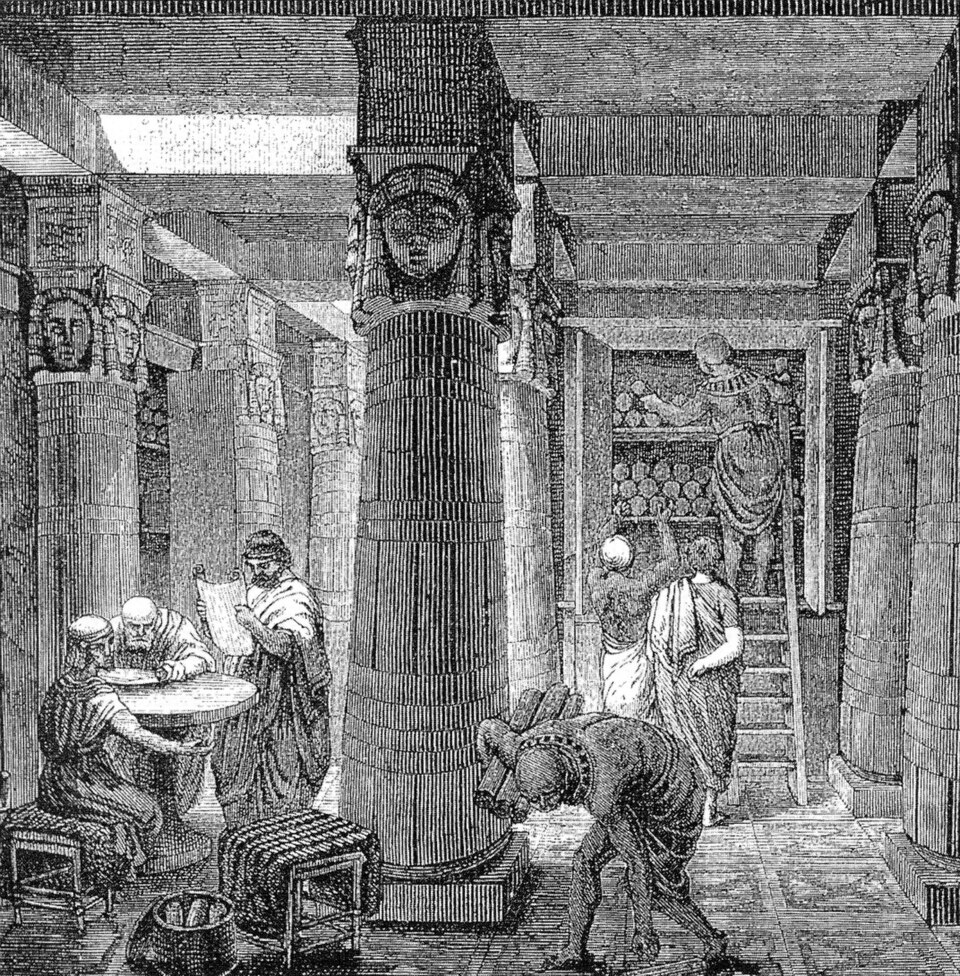
\includegraphics{images/misc/Ancientlibraryalex.jpg}
    \caption[Artistic Depiction of the Library of Alexandria based on historical evidence]{Artistic Depiction of the Library of Alexandria based on historical evidence. O. Von Corven -  "The Great Library of Alexandria"}

    % Latencies indicated in the figure are computed on the same machine \texttt{g2-standard-16} with a NVIDIA-L4 GPU, and averaged over 100 pages. Further details in \autoref{subsection:latency}.The computed score is the average of from all datasets in \textit{ViDoRe} for PDF Parser + Captioning and ColPali respectively. Further details in \autoref{section:results}.} 
    \label{fig:alexandria}
\end{marginfigure}

Long before computers, humans developed methods to organize and retrieve information. One of the earliest examples is the \emph{Pinakes} of Callimachus around the 3rd century BCE, often considered the first library catalog in the Western world. The \emph{Pinakes} is said to have systematically cataloged the authors and works held in the Library of Alexandria, organizing texts by subject and arranging authors alphabetically — an early bibliographic method that helped lay the foundations for later library catalogs. 

% This ancient effort demonstrated the enduring principles of indexing and categorization (such as alphabetical order and subject grouping) that remain fundamental in information retrieval (IR).


Through the centuries, librarians and scholars continued to develop catalogs and classification systems, from medieval manuscript indexes \sidecite{conraulewis_medieval_indices}
 to Melvil Dewey’s Decimal Classification in 1876 \sidecite{dewey1876classification}. These pre-digital innovations addressed the same core challenge as modern IR systems: \emph{how to store, organize, and find relevant information efficiently}. In 1945, Vannevar Bush articulated a technological vision for the future of information retrieval in \emph{As We May Think} \sidecite{bush1945aswemaythink}. He describes the inadequacy of indexing based systems to navigate the deluge of information:


\begin{lavenderkaobox}
"The real heart of the matter of selection, however, goes deeper than a lag in the adoption of mechanisms by libraries, or a lack of development of devices for their use. Our ineptitude in getting at the record is largely caused by the artificiality of systems of indexing. When data of any sort are placed in storage, they are filed alphabetically or numerically, and information is found (when it is) by tracing it down from subclass to subclass. It can be in only one place, unless duplicates are used; one has to have rules as to which path will locate it, and the rules are cumbersome."
\flushright -- Vannevar Bush, As We May Think (1945)
\end{lavenderkaobox}


Bush's vision was that new technology would enable moving away from this system. He proposes the \emph{Memex}, a hypothetical electromechanical desk that could instantly retrieve microfilmed documents via associative links. 
% Bush’s essay inspired later developments by suggesting that managing the “growing mountain of information” would require new mechanized solutions.

\section{Founding of Information Retrieval (1950s–1960s)}
Information Retrieval as a distinct field took shape in the 1950s and 1960s, alongside the advent of digital computers. In 1950, Calvin Mooers coined the term "information retrieval" \sidecite{mooers1950information}, heralding the idea of using machines to search document collections. Early experiments followed quickly: in 1951, a master’s thesis at MIT by Philip Bagley \sidecite{bagley1951electronic} demonstrated one of the first computerized document retrieval experiments. Pioneers like Hans Peter Luhn at IBM began applying computers to automate indexing; for example, Luhn developed methods for auto-encoding documents and keyword-in-context indexing. By 1959 he published an influential paper on “Auto-encoding of documents for information retrieval” \sidecite{luhn1959autoencoding} showing how computers could encode text and allow electronic searching of content. This period also saw growing support for IR research as the U.S. government recognized an information explosion funding projects on mechanized literature searching and the creation of citation indexes.


A key milestone was the Cranfield experiments led by Pete Cleverdon in the early 1960s \sidecite{cleverdon1967cranfield}. The Cranfield studies introduced a rigorous experimental methodology for IR: assembling a test collection of documents, queries, and relevance judgments, and evaluating retrieval performance using metrics like precision and recall. This methodology became a cornerstone of IR research, establishing a scientific approach to evaluate how “relevant” the results returned by an IR system are, laying the foundation for future benchmarks.
% The Cranfield approach was hard work (manually judging relevance for many query-document pairs), but it laid the foundation for future benchmarks.


During the same era, Gerard Salton formed the first major IR research group (at Harvard, later Cornell). Researchers began formulating the first theoretical models of IR. In 1960, Maron and Kuhns proposed a probabilistic indexing model \sidecite{maron1960relevance}, foreshadowing later probabilistic retrieval approaches. Salton and others started developing what became the vector space model: by the late 1960s, Salton’s team had created the SMART system, representing documents and queries as vectors in a term-weighted space. In 1968 Salton published “Automatic Information Organization and Retrieval” \sidecite{salton1968automatic} and by 1975 he fully articulated the vector space framework and term-weighting schemes \sidecite{salton1975vector_space}. Another 1960s contribution came from Karen Spärck Jones, who introduced the concept of inverse document frequency (IDF) \cite{sparck_jones_statistical_1972} to statistically downweight common terms and boost rare, informative terms – a principle that soon became central to ranking algorithms.

\section{The Statistical Revolution in IR (1970s--1990s)}

With the fundamentals laid, subsequent decades saw rapid improvement in statistical text retrieval methods. The 1970s refined the vector space and probabilistic models. Term frequency--inverse document frequency (TF--IDF) weighting became a standard technique: terms are scored higher if they appear frequently in a document (term frequency) but are rare across the collection (high IDF)\sidecite{sparck_jones_statistical_1972}\sidenote{
\textbf{TF-IDF:}
Let $\mathcal{D}=\{d_1,\dots,d_N\}$ be a corpus of $N$ documents and let $t$ be a term (token).
The TF--IDF weight of term $t$ in document $d$ is
\[
\mathrm{tfidf}(t,d,\mathcal{D}) \;=\; \mathrm{tf}(t,d)\cdot \mathrm{idf}(t,\mathcal{D}).
\]
A common choice is
\[
\mathrm{tf}(t,d)=\frac{f_{t,d}}{\sum_{t'} f_{t',d}}
\]
and
\[
\mathrm{idf}(t,\mathcal{D})=\log\!\left(\frac{N}{\mathrm{df}(t)}\right),
\]
where $f_{t,d}$ is the raw count of occurrences of $t$ in $d$, $\sum_{t'} f_{t',d}$ is the total number of term occurrences in $d$ (so $\mathrm{tf}$ is a normalized frequency),
and $\mathrm{df}(t)=\bigl|\{d_i\in\mathcal{D}: t\in d_i\}\bigr|$ is the document frequency (the number of documents containing $t$ at least once).
Intuitively, $\mathrm{tf}$ upweights terms frequent in a given document, while $\mathrm{idf}$ downweights terms that appear in many documents.
(Variants often use $\mathrm{tf}(t,d)=1+\log f_{t,d}$ and/or smoothing $\log\!\left(\frac{N+1}{\mathrm{df}(t)+1}\right)+1$ to avoid division by zero.)
}.  On the probabilistic side, Stephen Robertson and colleagues extended early ideas into the Probabilistic Relevance Framework in the 1970s and 1980s, leading to the development of ranking functions that estimate the probability a document is relevant to a query \sidecite{robertson1976relevance_weighting, robertson1977prp, robertson_probabilistic_2009}. These efforts culminated in the 1990s with Okapi BM25, developed in the Okapi/TREC line of work from the Robertson--Sp{\"a}rck Jones probabilistic framework and Robertson--Walker 2-Poisson approximations \sidecite{robertson1994bm25, robertson_okapi_1994}\sidenote{\textbf{BM25:}
Let $\mathcal{D}$ be a corpus, $d\in\mathcal{D}$ a document, and $t$ a term. The BM25 score of $d$ for a query $q$ is
\[
\mathrm{BM25}(q,d)=
\]
\[
\sum_{t\in q} \mathrm{idf}(t)\;
\frac{f_{t,d}(k_1+1)}{f_{t,d}+k_1\!\left(1-b+b\,\frac{|d|}{\mathrm{avgdl}}\right)}
\]
Here $f_{t,d}$ is the count of $t$ in $d$, $|d|$ is the document length (in tokens), and $\mathrm{avgdl}$ is the average document length in the corpus. $k_1>0$ controls term-frequency saturation, and $b\in[0,1]$ controls how strongly length normalization is applied. A common IDF is
\[
\mathrm{idf}(t)=\log\!\left(\frac{N-\mathrm{df}(t)+0.5}{\mathrm{df}(t)+0.5}\right),
\]
where $N=|\mathcal{D}|$ and $\mathrm{df}(t)$ is the number of documents containing $t$.
}. 
By incorporating TF--IDF-like features into a probabilistic model, BM25 became one of the dominant ranking algorithms in search and remains widely used as a strong baseline in modern information retrieval systems \sidecite{robertson_probabilistic_2009, manning2008introduction_ir}.

Alongside algorithm advances, IR systems grew in scale and importance. The first online search systems appeared in the early 1970s as databases of bibliographic records: for example, MEDLINE (1971) provided biomedical literature search, and DIALOG offered commercial online search over multiple databases \sidecite{nlm2024medline_history, dialog2019milestone}. These systems predated personal computers---users accessed them via terminals---but they demonstrated that searching thousands of documents via text queries was feasible and valuable. In 1978, the IR community established its premier conference, ACM SIGIR, reflecting the field's maturation \sidecite{sigir1978proceedings}.

By the 1980s, personal computing and CD-ROMs enabled standalone IR systems (like library catalog CDs), and researchers explored new ideas such as relevance feedback (the Rocchio algorithm from the 1970s allowed a system to adjust a query based on documents a user marked relevant) \sidecite{rocchio1971relevance_feedback} and clustering (the "cluster hypothesis": relevant documents tend to cluster together)\sidecite{jardine1971hierarchic_clustering, vanrijsbergen1979information_retrieval}. The inverted index (storing, for each term, a list of documents containing it) became a core data structure, enabling fast keyword lookup even as collections grew to tens of thousands of documents \sidecite{manning2008introduction_ir}. This era also saw experiments with user interfaces and visualization (e.g.\ plotting document similarity or using hypertext systems).

Evaluation at scale took a leap in 1992 with the start of the Text Retrieval Conference (TREC). TREC built large standard test collections and yearly competitions for state-of-the-art retrieval methods \sidecite{harman1993trec_overview}. TREC not only pushed research towards scalable methods but also fostered the development of specialized tasks. Many techniques that became important, such as query expansion and relevance feedback, were evaluated and refined through TREC workshops.

Web search emerged in the mid-1990s as a new frontier that dramatically expanded IR's scale and impact. Early web search systems and directories---for example, Yahoo!'s human-curated directory in 1994 and AltaVista in 1995---helped users navigate the growing World Wide Web, but human-maintained directories were difficult to scale and keyword-based engines often returned many low-quality matches at web scale\sidecite{brin1998anatomy}.

A major breakthrough came from the Stanford/Google work of the late 1990s, especially PageRank, which treated the web as a graph and used hyperlinks as an additional ranking signal: a page linked from many other pages, especially pages that were themselves important, received a higher importance score\sidecite{page1998pagerank, brin1998anatomy}. By combining link analysis with content relevance, anchor text, proximity, and other web-specific signals, Google produced more useful rankings than many earlier content-only systems\sidecite{brin1998anatomy}. This represented a graph-based retrieval innovation, leveraging network topology in a way analogous to citation analysis in scholarly literature.

In the 2000s, machine learning techniques became increasingly central to IR. Learning-to-rank algorithms learned how to combine many ranking features---such as lexical matching scores, anchor-text evidence, document features, and user-behavior-derived signals---into ranking functions\sidecite{burges2005ranknet, burges2006lambdarank, burges2010lambdamart}. Microsoft Research developed RankNet and LambdaRank in the mid-2000s, with LambdaMART later combining LambdaRank-style optimization with boosted decision trees\sidecite{burges2005ranknet, burges2006lambdarank, burges2010lambdamart}. Commercial search engines increasingly incorporated machine-learned ranking methods, although the exact algorithms and deployment timelines were often proprietary.

Researchers also showed that clickthrough logs and query reformulations could provide useful implicit feedback for ranking, though clicks are biased and must be interpreted carefully rather than treated as direct relevance judgments\sidecite{joachims2002clickthrough, joachims2005clickthrough, radlinski2005query_chains}.

Another 2000s-and-2010s trend was the use of semantic information and knowledge bases. For instance, Bing publicly described its Satori knowledge system in 2013 as modeling entities---people, places, and things---and relationships among them\sidecite{bing2013satori}. Google also moved in this direction through systems such as the Knowledge Graph and, in 2013, Hummingbird, a major improvement to its ranking systems associated with better handling of longer and more conversational queries\sidecite{google2025ranking_systems}.

\section{The Deep Learning Era of IR (2010s--2020s)}

The 2010s shifted information retrieval from purely lexical matching toward neural semantic matching. Early neural IR systems such as DSSM mapped queries and documents into learned vector spaces, allowing systems to match texts that used different words but expressed related meanings\sidecite{huang2013dssm}. This was the beginning of dense retrieval: instead of representing a document only by the terms it contains, the system learns a continuous embedding that captures semantic similarity.

The transformer era accelerated this shift. BERT showed that large pretrained language models could produce rich contextual representations of text,\sidecite{devlin2019bert} and by 2019 Google had publicly announced the use of BERT in Search to better handle longer, more conversational queries\sidecite{google2019bert_search}. In academic IR, BERT-style cross-encoders became especially effective as rerankers: a first-stage retriever such as BM25 or a dense retriever retrieves a candidate set, and a neural model then scores each query--document pair more precisely\sidecite{nogueira_passage_2019, yates2021transformers_ranking}.

At the same time, researchers developed neural retrievers that could operate efficiently at first stage. Bi-encoders or dual encoders represent queries and documents independently, so retrieval can be performed through nearest-neighbor search in vector space\sidecite{karpukhin2020dpr}. Sentence-BERT made BERT-style sentence embeddings practical for semantic similarity and retrieval,\sidecite{reimers2019sbert} while DPR showed that dense passage retrieval could outperform BM25 on several open-domain question-answering benchmarks\sidecite{karpukhin2020dpr}. Late-interaction models such as ColBERT offered a middle ground: they retained token-level matching signals while remaining much more efficient than full cross-encoder reranking\sidecite{khattab2020colbert}.

By the early 2020s, the dominant neural IR architecture had become multi-stage: a fast lexical, sparse, or dense retriever produces candidates; a stronger neural reranker refines them; and systems often combine lexical and semantic signals rather than replacing one with the other\sidecite{yates2021transformers_ranking}.



\section{The Modern Stack: Hybrid, Contextual, and Agentic Retrieval}

Modern IR is no longer a simple competition between BM25 and dense vectors. High-performing systems increasingly combine multiple retrieval signals: lexical matching for exact terms, dense embeddings for semantic similarity, learned sparse models for interpretable expansion, late-interaction models for token-level matching, and cross-encoders or LLM rerankers for final precision.

A first trend is the rise of general-purpose embedding models. Models such as GTE train unified text embeddings with multi-stage contrastive learning over diverse datasets,\sidecite{li2023generaltextembeddingsmultistage} while E5-style models and E5-Mistral show that strong embedding models can be built by adapting large language models and training on large synthetic instruction-style data\sidecite{wang2024improvingtextembeddingslarge}. More recent work directly adapts decoder-only LLMs into embedding models: LLM2Vec converts causal LLMs into bidirectional text encoders through bidirectional attention, masked next-token prediction, and contrastive learning,\sidecite{behnamghader_llm2vec_2024} while NV-Embed introduces practical techniques such as latent-attention pooling, removing the causal mask during contrastive training, and two-stage instruction tuning\sidecite{lee2024nvembedimprovedtechniquestraining}. NV-Retriever further highlights the importance of hard-negative mining, especially positive-aware methods that reduce false negatives during contrastive learning\sidecite{moreira2024nvretriever}.

A second trend is the return of sparse retrieval in neural form. Learned sparse models preserve the operational advantages of inverted indexes while learning term expansion and weighting from data. SPLADE is a representative example: it learns sparse lexical representations using explicit sparsity regularization and log-saturated term weights, making it suitable for first-stage retrieval with inverted indexes\sidecite{10.1145/3404835.3463098}. More recent work pushes this idea beyond vocabulary terms. Sparse-autoencoder-based retrieval models such as SPLARE learn sparse latent embeddings from LLM representations, aiming for more semantic and multilingual sparse features\sidecite{formal2026learningretrievalmodelssparse}. The Latent Terms line of work similarly shows that dense retrievers can contain extractable sparse, BM25-ready latent features, suggesting that dense and sparse retrieval may be less separate than they first appear\sidecite{latentterms}.

A third trend concerns context. Standard chunking pipelines often split documents before embedding them, which can remove surrounding context from each chunk. Late Chunking reverses this order: it first encodes a longer text with a long-context embedding model, then pools token representations into chunk embeddings, allowing chunk vectors to retain information from the broader document\sidecite{LateChunking}. Contextual Document Embeddings extend the same idea to corpora: a document representation can be improved by considering neighboring or related documents rather than encoding each document in isolation\sidecite{morris2024contextualdocumentembeddings}. This matters especially for RAG systems, where the quality of retrieved chunks can depend on information outside the chunk itself.

A fourth trend is more expressive scoring. Dense retrieval usually scores a query and document by a dot product or cosine similarity between vectors, which is efficient but limits the kinds of relevance functions that can be represented. Hypencoder proposes a different paradigm: the query encoder produces a small neural network that scores document representations, allowing query-specific relevance functions while still supporting approximate retrieval\sidecite{killingback2025hypencoderhypernetworksinformationretrieval}. This illustrates a broader movement beyond fixed-vector similarity toward richer, task-adaptive scoring mechanisms.

Finally, retrieval is becoming agentic and reasoning-aware. Classical search assumes a user issues a query and receives a ranked list. Modern LLM-based systems often plan, decompose a task, issue multiple searches, inspect evidence, and reformulate queries. ReasonIR trains retrievers specifically for reasoning-intensive tasks, using synthetic data that pairs challenging queries with relevant documents and hard negatives\sidecite{shao2025reasonir}. AgentIR goes further by treating deep-research agents as retrieval users: instead of embedding only the final query, it embeds the agent's reasoning trace together with the query, so the retriever can exploit the agent's expressed intent\sidecite{chen2026agentir}. In this view, IR is no longer just document ranking; it becomes part of a larger reasoning loop involving query planning, retrieval, reranking, evidence synthesis, and attribution.


% \section{Engineering}
% FAISS,

% \section{Industrial Applications}

% RAG, word extraction
